\section{Differential Dynamic Microscopy}\label{sec:DDMDis}
The measured datasets were evaluated using a provided matlab script, which first calculated the dynamic structure function $D(q,\Delta t)$ for exponential increasing time differences $\Delta t$. Therefore, the difference intensities 
\begin{equation}
    \Delta I(x,y,\Delta t) = I(x,y,t+\Delta t) - I(x,y,t)
\end{equation}
were transformed into the fourier space intensities $\Delta I(q_x,q_y,\Delta t)$ using a 2d fast fourier trasform algorithm. $D(q,\Delta t)$ is obtained by averiging radial over the dynamic structure function 
\begin{equation}
    D(q_x,q_y,\Delta t) = \langle |\Delta I(x,y,\Delta t)|^2 \rangle.
\end{equation}
Resulting plots of $D(q_x,q_y,\Delta t)$ for selected $q$ can be seen in fig.~\ref{fig:DvsDeltat}. Hereby can be seen, that especially for small $q$ increasing $\Delta t$ lead to bigger noise and poor statistics. Therefore, a cutoff for $\Delta t$ was set manually. \par 

\begin{figure}[ht]
    \centering
    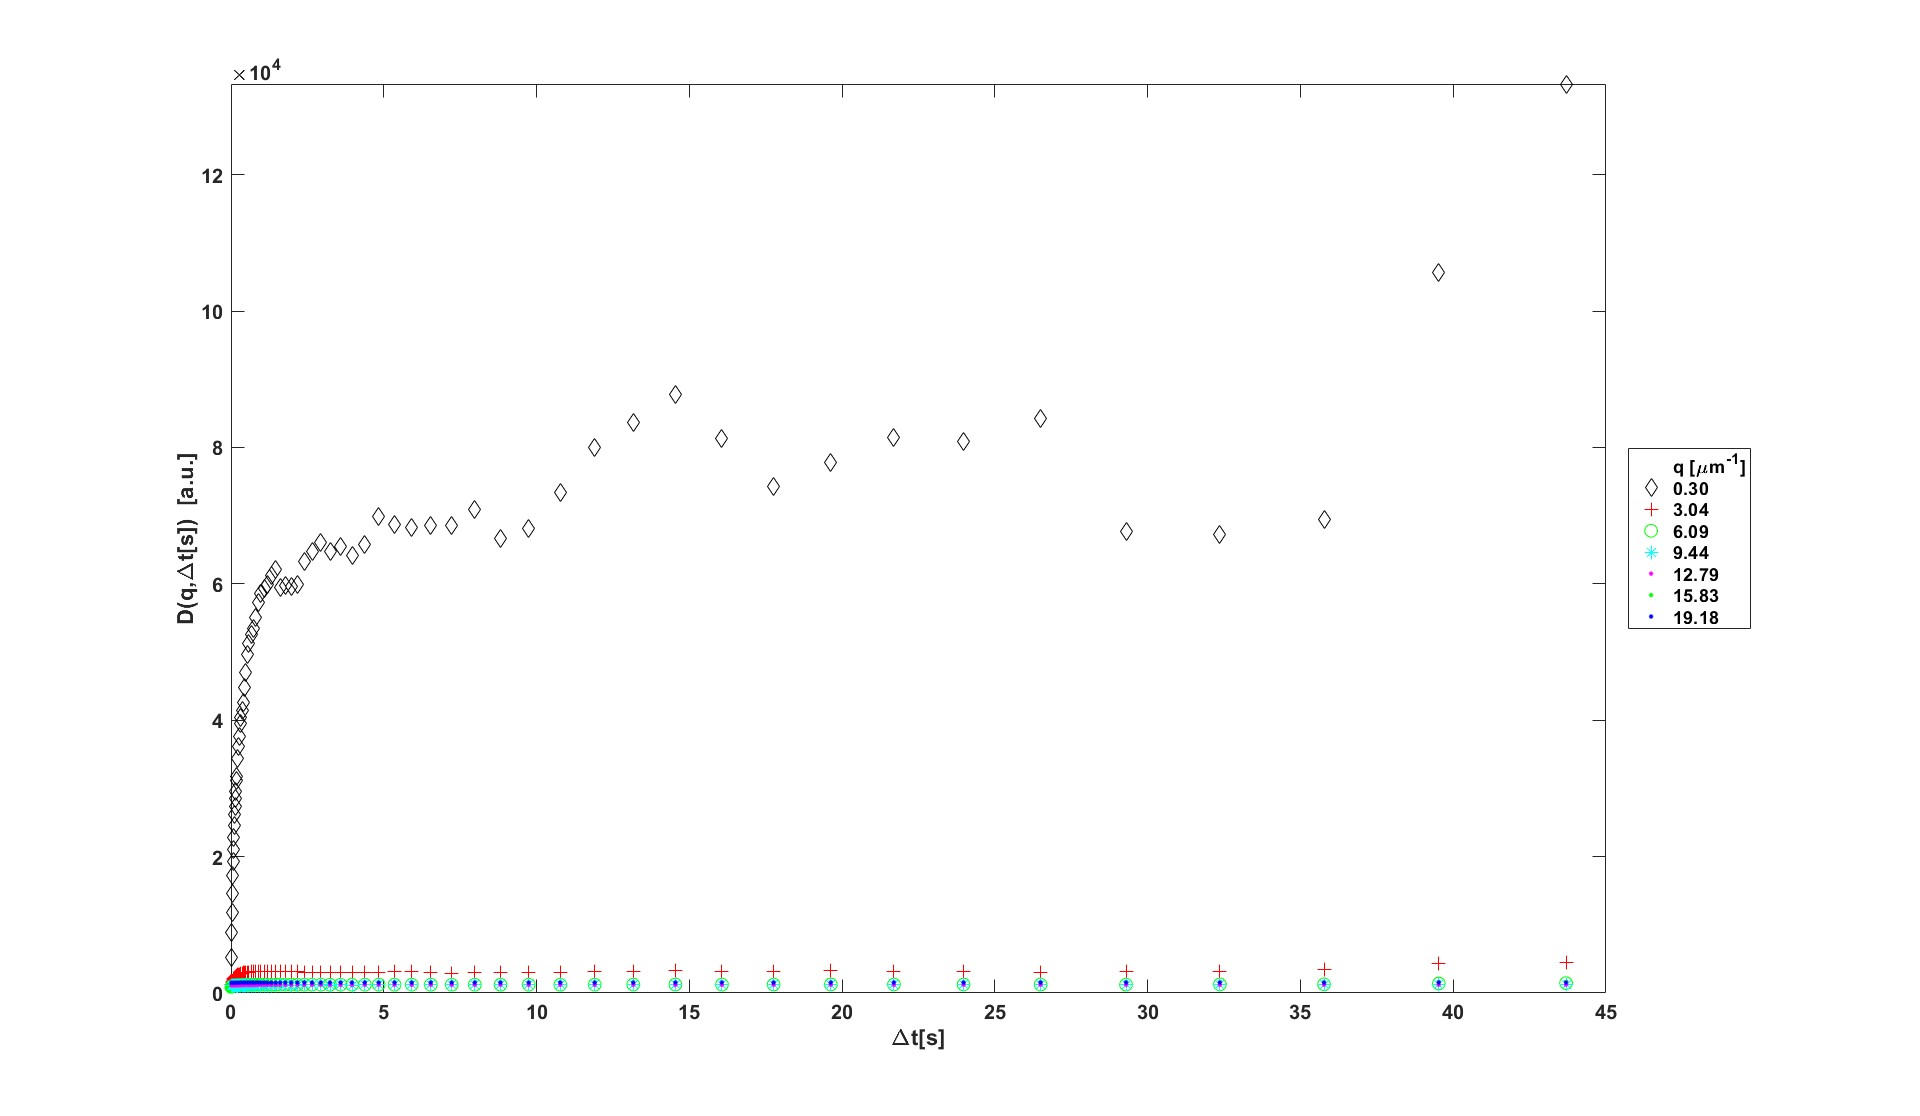
\includegraphics[width = \textwidth]{Bilder/Auswertung/DDM/d vs detat.jpg}
    \caption{The calculated dynamic structure function $D(q_x,q_y,\Delta t)$ is plotted against $\Delta t$ for selected $q$. For small $q$ an increasing $\Delta t$ leads to bigger noise and poor statistics.}
    \label{fig:DvsDeltat}
\end{figure}

As the dynamic structure function is expected to follow eq.~\ref{eq:21.3}, a fit was made, obtaining $A(q)$, $B(q)$ and $\tau (q)$. Eq.~\ref{eq:21.4} states 
\begin{equation}
    \tau (q) \propto q^{-2}
\end{equation}
and therefore the log-log-plot of $\tau (q)$ against $q$ should be a straight line with slope \num{-2}. As can be seen in fig.~\ref{fig:tauvsQ}, this is not the case for too small or too big $q$. Consequently a range for $q$ for the application of the fit of eq.~\ref{eq:21.4} was set. In this way, for each dataset a value for $D_m$ was obtained. As for every configuration of the setup five measurements were done, the $D_m$ were averaged afterwards. The results are stated in tab.~\ref{tab:Dm}.

\begin{figure}[ht]
    \centering
    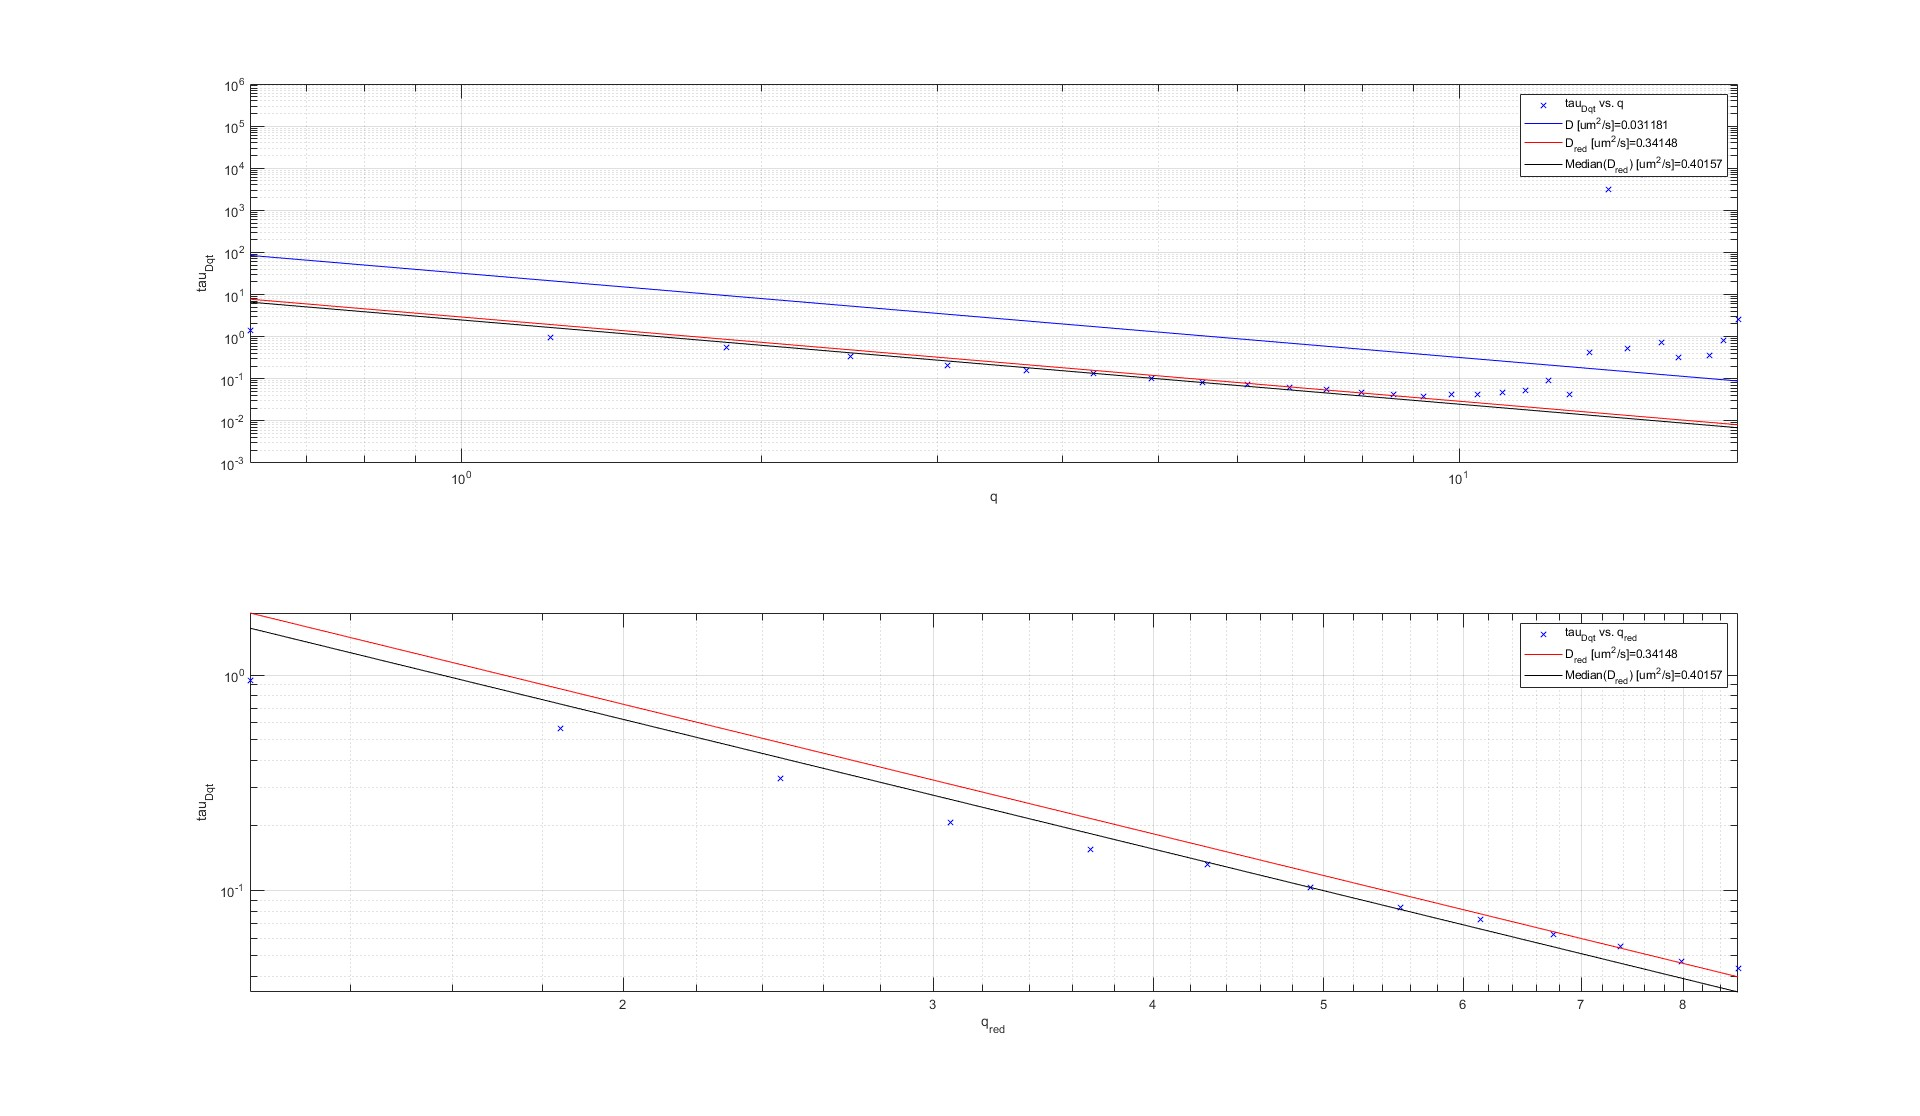
\includegraphics[width = \textwidth]{Bilder/Auswertung/DDM/tauvsQ.jpg}
    \caption{The values for $\tau (q)$ obtained from the fits were plotted against $q$ (upper plot). Too small and too big $q$ do not follow eq.~\ref{eq:21.4} and therefore lead to a wrong value for $D_m$ (fit in blue). Cosequently, the fit is only applied to a manually defined reduced $q$ space (lower plot and fits in red and black).}
    \label{fig:tauvsQ}
\end{figure}

\begin{table}
    \centering
    \begin{tabular}{c c c | c}
        \toprule
        binning & ROI size / \si{\micro\meter} & pinhole & $D_m$ / \si{\micro\meter^2 \per\second}
    \end{tabular}
    \label{tab:Dm}
\end{table}